\section{Redes Neuronales de Impulsos}

\subsection{¿Qué es una Red Neuronal de Impulsos?}

Las redes neuronales que conocemos, las ANNs tradicionales, procesan información usando números continuos. Cada neurona recibe valores como 0.87 o 0.34, los procesa, y produce otro número continuo. Pero así no es como trabaja el cerebro real.

Las SNNs funcionan de manera diferente. En lugar de transmitir valores numéricos continuos, estas redes se comunican mediante impulsos breves de actividad eléctrica llamados impulsos igual que las neuronas biológicas. Un impulso es un evento discreto: la neurona dispara o no dispara.

Pensemos en una analogía: una ANN tradicional se parece a un termostato analógico que ajusta gradualmente la temperatura en un rango continuo de valores. Una SNN, en cambio, funciona más como un sistema de código Morse: transmite información mediante impulsos discretos que ocurren en momentos específicos del tiempo. El mensaje no está solo en si hay impulso o no, sino también en cuándo ocurre.

\subsubsection{Diferencias fundamentales con las ANNs tradicionales}

La tabla \ref{tab:ann-vs-snn} resume las diferencias principales entre ambos paradigmas:

\begin{table}[htbp]
\centering
\begin{tabular}{p{4cm}p{5cm}p{5cm}}
\hline\hline
\textbf{Aspecto} & \textbf{ANN Tradicional} & \textbf{SNN} \\
\hline
Comunicación entre neuronas & Valores continuos (0.0 - 1.0) & Impulsos discretos (impulso/no impulso) \\
\hline
Información temporal & El momento exacto no importa & El TIEMPO del impulso es información \\
\hline
Activación & Cada neurona procesa en cada paso & Solo procesa cuando recibe un impulso \\
\hline
Operaciones & Multiplicaciones intensivas & Sumas y comparaciones \\

\hline\hline
\end{tabular}
\caption{Comparación entre ANNs tradicionales y SNNs}
\label{tab:ann-vs-snn}
\end{table}

% En una ANN tradicional, si tenemos tres neuronas conectadas secuencialmente, el flujo de información podría verse así:
% \begin{center}
% \texttt{Neurona A (0.7) → Neurona B (0.4) → Neurona C (0.9)}
% \end{center}

% Cada neurona transmite un valor numérico continuo. El tiempo no juega ningún papel: da igual si esos valores se calculan en el instante $t=1$ o en $t=100$.

% En una SNN con la misma topología, el flujo es diferente:
% \begin{center}
% \texttt{Neurona A (spike en t=3) → Neurona B (spike en t=5) → Neurona C (sin spike)}
% \end{center}

% Aquí las neuronas se comunican mediante eventos discretos que ocurren en momentos específicos. La neurona A dispara un impulso en el instante $t=3$, lo cual causa que la neurona B acumule carga y eventualmente dispare en $t=5$. La neurona C, en cambio, no alcanza el umbral necesario para disparar. Esta dinámica temporal es esencial para entender cómo operan las SNNs.

% La consecuencia más importante de este diseño es que las SNNs son impulsadas por eventos. La mayoría de las neuronas están inactivas la mayor parte del tiempo, despertándose solo cuando reciben un impulso. Esto contrasta con las ANNs, donde todas las neuronas calculan activamente en cada paso temporal, consuman o no esa información.

% \subsection{Componentes básicos de una SNN}

% Ahora que entendemos el concepto general, veamos las piezas que conforman una SNN y cómo funcionan.

% \subsubsection{La neurona de impulsos: modelo LIF}

% El tipo de neurona más común en SNNs se llama LIF. A continuación se explican los componentes clave de este modelo:

% \begin{itemize}
%     \item \textbf{Fuga:} El voltaje no se mantiene indefinidamente. Si la neurona no recibe más entradas, el voltaje decae gradualmente con el tiempo, como si hubiera una fuga de carga.
%     \item \textbf{Integración:} La neurona acumula las señales eléctricas que recibe. Cada vez que llega un impulso desde otra neurona, el voltaje de membrana aumenta.
%     \item \textbf{Disparo:} Cuando el voltaje acumulado supera un umbral determinado, la neurona emite su propio impulso y su voltaje se reinicia a un valor de reposo.
% \end{itemize}

% Podemos expresar esta dinámica con una ecuación simple:
% \begin{equation}
%     V(t+1) = V(t) \times \text{decay} + \text{impulso\_recibidos}
% \end{equation}

% Si $V(t+1) \geq \text{threshold}$, entonces la neurona dispara un impulso y $V$ se reinicia a $V_{\text{rest}}$.

% Los parámetros clave son:
% \begin{itemize}
%     \item $V(t)$: voltaje de la membrana neuronal en el instante $t$ (típicamente en milivoltios, mV)
%     \item decay: factor de decaimiento (por ejemplo, 0.95 significa que la neurona pierde 5\% de su voltaje por paso temporal si no recibe entradas)
%     \item threshold: umbral de disparo (por ejemplo, $-50$ mV)
%     \item $V_{\text{rest}}$: voltaje de reposo al que vuelve después de disparar (por ejemplo, $-65$ mV)
% \end{itemize}

% Un ejemplo concreto ayuda a visualizar el proceso. Supongamos una neurona LIF con los siguientes parámetros:
% \begin{itemize}
%     \item $V_{\text{rest}} = -65$ mV
%     \item threshold $= -50$ mV
%     \item decay $= 0.95$
% \end{itemize}

% En $t=0$, la neurona está en reposo: $V(0) = -65$ mV. En $t=1$, recibe un impulso con peso $+8$ mV, así que:
% \[
% V(1) = -65 \times 0.95 + 8 = -61.75 + 8 = -53.75 \text{ mV}
% \]

% El voltaje subió, pero aún está por debajo del umbral ($-50$ mV), así que no dispara. En $t=2$, no recibe más entradas, entonces:
% \[
% V(2) = -53.75 \times 0.95 = -51.06 \text{ mV}
% \]

% El voltaje decae lentamente. Si en $t=3$ recibe otro impulso de $+5$ mV:
% \[
% V(3) = -51.06 \times 0.95 + 5 = -48.51 + 5 = -43.51 \text{ mV}
% \]

% ¡Ahora $V(3) > -50$ mV! La neurona supera el umbral, emite un impulso, y su voltaje se reinicia: $V(3) \rightarrow -65$ mV.

% Este ciclo se repite continuamente. El diagrama temporal del voltaje mostraría algo así:

% \begin{verbatim}
% Voltaje (mV)
%     -40 |         *  (spike!)
%         |        /|
%     -50 |- - - - - - - - - (threshold)
%         |       / |
%     -60 |------   |
%         |     /   |
%     -65 |----     -------- (reset)
%         |_____________________
%            t=1  t=2  t=3  t=4
%               tiempo →
% \end{verbatim}

% La simplicidad del modelo LIF es una de sus mayores ventajas. Captura la dinámica esencial de las neuronas biológicas sin requerir ecuaciones diferenciales complejas, lo que permite simulaciones eficientes.


\subsection{Componentes básicos de una SNN}

Ahora que entendemos el concepto general, veamos las piezas que conforman una SNN y cómo funcionan.

\subsubsection{La neurona de impulsos: modelo LIF}

El tipo de neurona más común en SNNs se llama LIF. A continuación se explican los componentes clave de este modelo:

\begin{itemize}
    \item \textbf{Fuga:} El voltaje no se mantiene indefinidamente. Si la neurona no recibe más entradas, el voltaje decae gradualmente con el tiempo, como si hubiera una fuga de carga.
    \item \textbf{Integración:} La neurona acumula las señales eléctricas que recibe. Cada vez que llega un impulso desde otra neurona, el voltaje de membrana aumenta.
    \item \textbf{Disparo:} Cuando el voltaje acumulado supera un umbral determinado, la neurona emite su propio impulso y su voltaje se reinicia a un valor de reposo.
\end{itemize}

En la literatura, la dinámica del modelo LIF se describe normalmente mediante una ecuación diferencial continua \cite{gerstner2014neuronal, dayan2001theoretical}:

\begin{equation}
C_m \frac{dV(t)}{dt} = -g_L \big(V(t) - E_L\big) + I_{\text{syn}}(t)
\label{eq:lif-continuo}
\end{equation}

donde $C_m$ es la capacitancia de membrana, $g_L$ la conductancia de fuga, $E_L$ el voltaje de reposo, e $I_{\text{syn}}(t)$ la corriente sináptica de entrada.

Para simplificar las simulaciones, es habitual usar una versión discreta del modelo, que aproxima la ecuación anterior en pasos temporales:

\begin{equation}
V(t+1) = V(t) + \alpha \big(V_{\text{rest}} - V(t)\big) + I_{\text{entrada}}(t)
\label{eq:lif-discreto}
\end{equation}
  
Si $V(t+1) \geq V_{\text{threshold}}$, la neurona dispara un impulso y se reinicia a $V_{\text{rest}}$.

Los parámetros principales son:

\begin{itemize}
    \item $V(t)$: voltaje de la membrana en el instante $t$ (unidad de medida: milivoltios, mV)
    \item $\alpha$: factor de fuga, donde $0 < \alpha < 1$. \alpha$ controla la rapidez con que el voltaje tiende hacia el reposo (por ejemplo, 0.2 indica que el voltaje recupera un 20\% de la diferencia hacia el reposo por paso temporal)
    \item $V_{\text{rest}}$: voltaje de reposo (por ejemplo, $-65$ mV)
    \item $V_{\text{threshold}}$: umbral de disparo (por ejemplo, $-50$ mV)
    \item $I_{\text{entrada}}(t)$: representa el efecto total de los impulsos recibidos en el instante $t$.
\end{itemize}

\paragraph{Ejemplo ilustrativo.} Supongamos una neurona LIF con los siguientes parámetros:

\begin{itemize}
    \item $V_{\text{rest}} = -65$ mV
    \item $V_{\text{threshold}} = -50$ mV
    \item $\alpha = 0.2$
\end{itemize}

En $t=0$, la neurona está en reposo: $V(0) = -65$ mV.  
En $t=1$, recibe un impulso de $+20$ mV. El término de fuga es:

\[
\text{$\alpha$} = 0.2 \times (-65 - (-65)) = 0
\]
\[
V(1) = -65 + 0 + 20 = -45 \text{ mV}
\]

El voltaje supera el umbral ($-50$ mV), por lo que la neurona dispara un impulso y se reinicia: $V(1) \rightarrow -65$ mV.

Si en $t=2$ recibe un impulso de $+10$ mV:

\[
\text{$\alpha$} = 0.2 \times (-65 - (-65)) = 0
\]
\[
V(2) = -65 + 0 + 10 = -55 \text{ mV}
\]

El voltaje no alcanza el umbral.  
En $t=3$, sin nuevas entradas, el voltaje decae:

\[
\text{$\alpha$} = 0.2 \times (-65 - (-55)) = -2 \text{ mV}
\]
\[
V(3) = -55 + (-2) + 0 = -57 \text{ mV}
\]

En $t=4$, recibe un nuevo impulso de $+10$ mV:

\[
\text{$\alpha$} = 0.2 \times (-65 - (-57)) = -1.6 \text{ mV}
\]
\[
V(4) = -57 + (-1.6) + 10 = -48.6 \text{ mV}
\]

Como $V(4) > -50$ mV, la neurona dispara y se reinicia a $V_{\text{rest}} = -65$ mV.

El proceso se repite en cada paso temporal, dando lugar a un patrón de disparos como el que se muestra en la Figura \ref{fig:voltaje-neurona-lif}:

\begin{figure}[!htb]
    \centering
    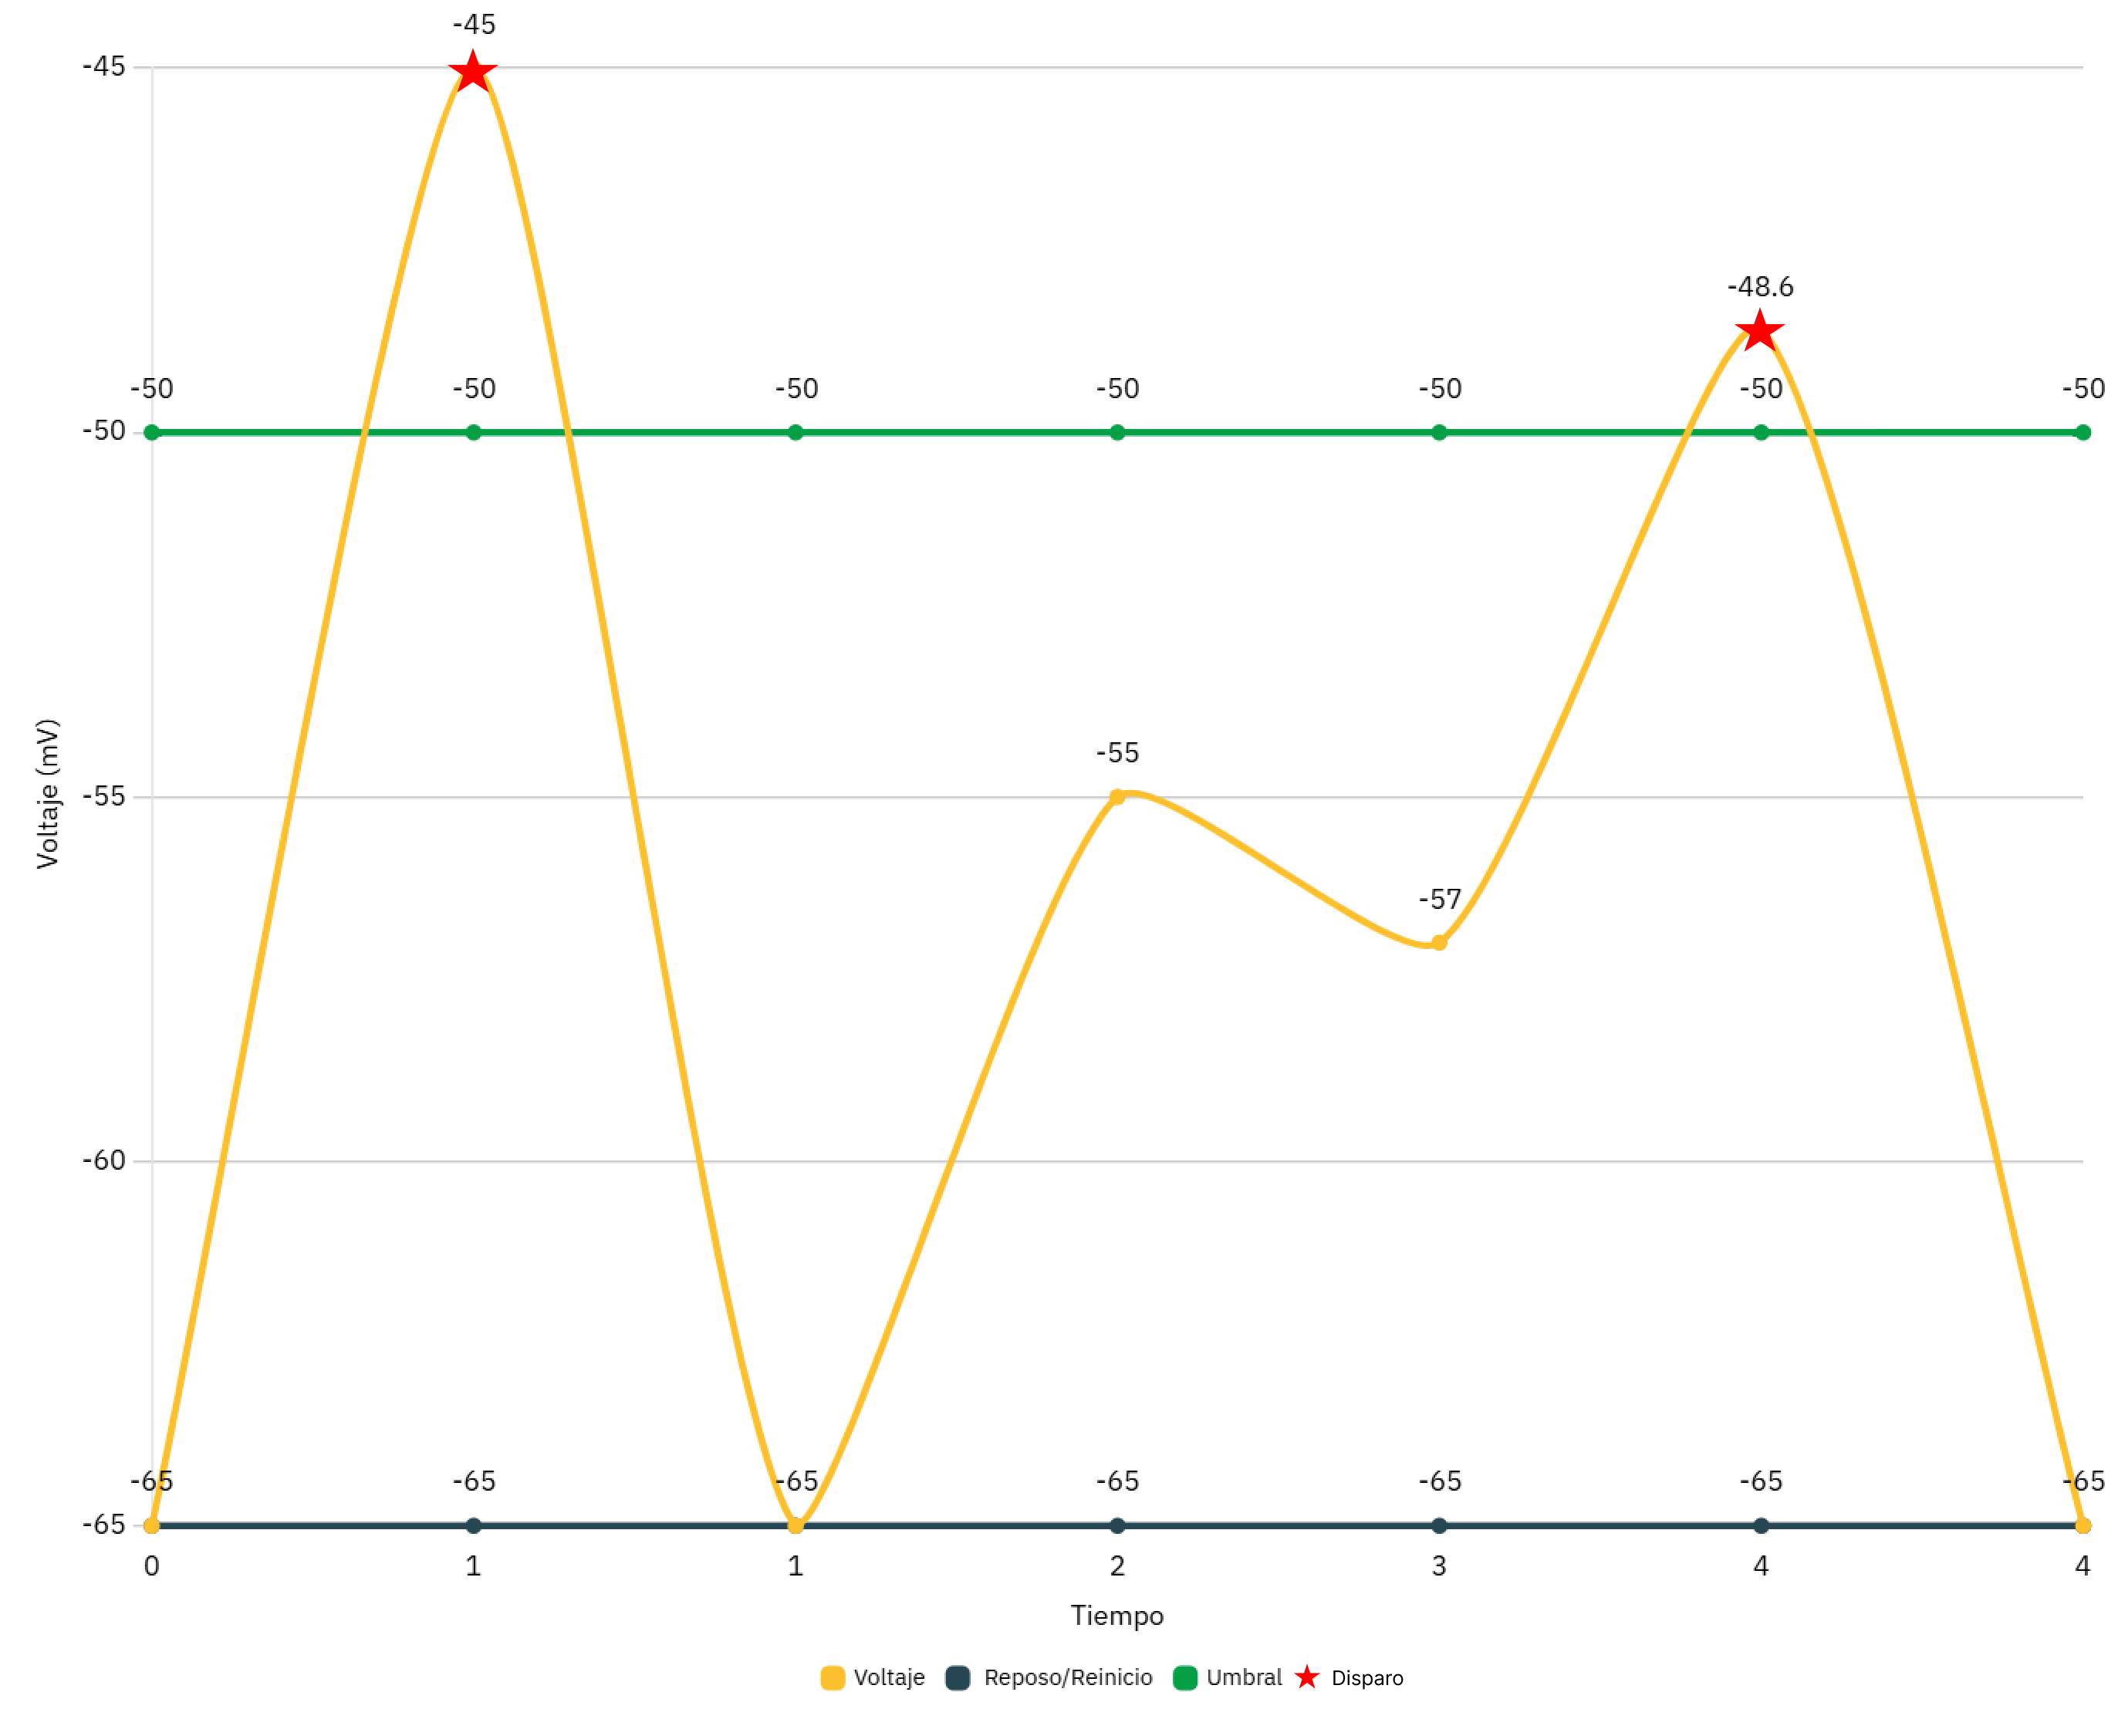
\includegraphics[width=1.0\textwidth]{Imagenes/Ejemplo ilustrativo de una neurona LIF.png}
    \caption{Ejemplo ilustrativo de una neurona LIF. Fuente: Elaboración propia.}
    \label{fig:voltaje-neurona-lif}
\end{figure}

La simplicidad del modelo LIF es una de sus mayores ventajas: permite capturar la dinámica esencial del disparo neuronal sin recurrir a ecuaciones diferenciales complejas, lo que lo hace ideal para simulaciones eficientes.


\subsubsection{Sinapsis: las conexiones entre neuronas}

Cuando una neurona dispara un impulso, este no llega automáticamente a todas las demás neuronas. Viaja a través de sinapsis, las conexiones entre neuronas. Cada sinapsis tiene un peso sináptico que determina cuánto impacto tiene el impulso en la neurona receptora.

Los pesos pueden ser de dos tipos:
\begin{itemize}
    \item \textbf{Positivos (excitatorios):} Aumentan el voltaje de la neurona receptora, haciéndola más propensa a disparar.
    \item \textbf{Negativos (inhibitorios):} Disminuyen el voltaje, haciendo menos probable que dispare.
\end{itemize}

Veamos un ejemplo concreto. Supón que la neurona A dispara un impulso y está conectada a la neurona B mediante una sinapsis con peso $+0.5$. Cuando el impulso llega, la neurona B recibe un incremento de voltaje de $+0.5$ mV. Si esa misma sinapsis tuviera un peso de $-0.3$, la neurona B experimentaría una disminución de $-0.3$ mV en su voltaje.

Esta interacción entre excitación e inhibición es fundamental. Las neuronas excitatorias activan a otras neuronas, propagando información. Las neuronas inhibitorias, en cambio, actúan como frenos, evitando que la red se sature con actividad descontrolada. El balance entre ambas determina la estabilidad y el comportamiento de la red.

\subsection{Arquitectura SNN base para detección de anomalías en series temporales}

Una vez comprendidos los fundamentos de las SNNs, en esta sección se describe la arquitectura SNN base, específicamente diseñada para la detección de anomalías en series temporales, que constituye el punto de partida para la solución propuesta en el Capítulo \ref{chap:especificacion}.

% \subsubsection{Motivación y principio de funcionamiento}

% La hipótesis fundamental de este enfoque es que una SNN entrenada con datos normales mediante STDP exhibirá patrones de disparo característicos al procesar dichos datos. Cuando la red se enfrenta a datos anómalos o con comportamientos diferentes a los aprendidos, los patrones de disparo cambiarán significativamente. Específicamente, se espera que la frecuencia de generación de impulsos sea distinta al procesar datos normales frente a datos anómalos.

% Esta aproximación aprovecha las propiedades inherentes de las SNNs: su capacidad de aprendizaje no supervisado mediante STDP y su sensibilidad a los patrones temporales de la información de entrada.

\subsubsection{Arquitectura bicapa}

El modelo SNN base consta de dos capas principales, denominadas A y B:

\paragraph{Capa A (entrada).} Esta capa actúa como interfaz entre los datos de entrada y la red neuronal. Su función es transformar los valores continuos de la serie temporal en impulsos discretos. El número de neuronas en esta capa es 39.

\paragraph{Capa B (procesamiento).} Compuesta por 100 neuronas LIF completamente conectadas a la capa A. Esta capa presenta dos características distintivas:

\begin{itemize}
    \item Conexiones feedforward desde la capa A: cada neurona de la capa B recibe entradas ponderadas desde todas las neuronas de la capa A.
    \item Conexiones recurrentes dentro de la propia capa B: las neuronas están interconectadas entre sí, permitiendo que los impulsos generados en esta capa influyan en el estado de las demás neuronas del mismo nivel. Estas conexiones recurrentes son fundamentales para capturar dependencias temporales en los datos.
\end{itemize}

\begin{figure}[!htb]
    \centering
    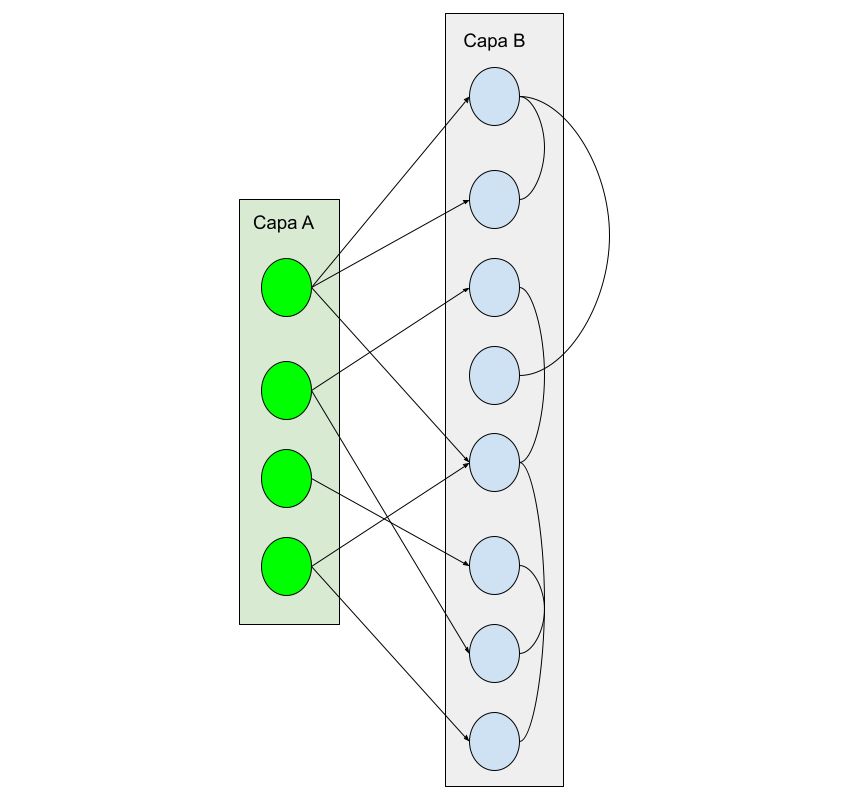
\includegraphics[width=0.8\textwidth]{Imagenes/Diagrama de capas de SNN Base.png}
    \caption{Diagrama de la arquitectura bicapa de la SNN base. Fuente: Iago.}
    \label{fig:arquitectura-bicapa-snn}
\end{figure}

\subsubsection{Codificación por cuantiles}

Para convertir valores continuos de series temporales en impulsos discretos, se emplea una estrategia de codificación basada en cuantiles estadísticos. Este método divide el rango de valores observados en el conjunto de entrenamiento en intervalos disjuntos, donde cada intervalo corresponde a una neurona de la capa A.

El proceso funciona de la siguiente manera:

\begin{enumerate}
    \item Durante la fase de preparación, se calculan los cuantiles de la distribución de valores en los datos de entrenamiento. Por ejemplo, si se eligen $n$ cuantiles, se obtienen $n-1$ neuronas en la capa A.
    \item Cada valor de la serie temporal se asigna al intervalo que le corresponde según su magnitud.
    \item La neurona asociada a dicho intervalo genera un impulso en el instante temporal actual.
    \item Este impulso se propaga a la capa B a través de las conexiones sinápticas.
\end{enumerate}

Esta codificación presenta ventajas importantes: es determinista, computacionalmente eficiente y adapta automáticamente la representación a la distribución estadística de los datos específicos del problema. Además, valores fuera del rango original pueden ser manejados mediante intervalos adicionales en los extremos.

\subsubsection{Aprendizaje mediante STDP modificado}

El entrenamiento de la red se realiza mediante una variante de STDP diseñada específicamente para la tarea de detección de anomalías. A diferencia del STDP clásico, donde se refuerzan conexiones que conducen a disparos postsinápticos inmediatos, aquí se emplea una estrategia de penalización bidireccional.

El mecanismo funciona de la siguiente forma:

\begin{itemize}
    \item Se penalizan las conexiones hacia neuronas que hayan emitido impulsos recientemente (impulsos presinápticos).
    \item También se penalizan las conexiones hacia neuronas que disparen inmediatamente después del impulso actual (impulsos postsinápticos).
\end{itemize}

Esta doble penalización tiene como objetivo inhibir la generación de impulsos cuando la red procesa datos normales, es decir, datos similares a los observados durante el entrenamiento. La intuición es que, si la red ha aprendido correctamente los patrones normales, debería generar pocos impulsos al encontrarlos nuevamente. En cambio, ante datos anómalos, las conexiones ajustadas no serán efectivas para suprimir la actividad, resultando en un mayor número de impulsos.

Los parámetros de aprendizaje nu1 y nu2 controlan la magnitud de los ajustes sinápticos en las conexiones A→B y B→B respectivamente. Estos valores son típicamente negativos para implementar la penalización descrita.

\subsubsection{Criterio de detección de anomalías}

Una vez entrenada la red, la detección de anomalías se basa en la frecuencia de impulsos generados por la capa B durante la inferencia. El procedimiento es el siguiente:

\begin{enumerate}
    \item Durante el procesamiento de nuevos datos, se monitoriza la actividad de disparo de las neuronas en la capa B.
    \item Se calcula una métrica agregada de la actividad neuronal, típicamente la suma de impulsos en una ventana temporal deslizante.
    \item Esta señal de actividad se suaviza mediante técnicas como media móvil para reducir fluctuaciones instantáneas.
    \item Se compara la actividad suavizada con un umbral estadístico predeterminado.
    \item Cuando la actividad supera el umbral, se genera una alerta de anomalía.
\end{enumerate}

El umbral puede establecerse mediante análisis estadístico de la actividad observada durante el procesamiento de datos de validación normales, por ejemplo, utilizando la media más dos desviaciones estándar.

\subsubsection{Limitaciones de la arquitectura base}

Aunque esta arquitectura demuestra la viabilidad de aplicar SNNs a la detección de anomalías, presenta varias limitaciones que motivan el desarrollo de mejoras:

\begin{itemize}
    \item Ausencia de extracción de características jerárquicas: la conectividad completamente conectada (fully-connected) no captura eficientemente patrones locales o estructuras temporales específicas, que son fundamentales para detectar anomalías sutiles en series temporales complejas.
    
    \item Sensibilidad a hiperparámetros: los parámetros nu1, nu2, el umbral de disparo y la constante de decaimiento deben ajustarse manualmente o mediante búsqueda exhaustiva, sin un mecanismo de optimización automatizada.
    
    \item Rendimiento limitado en presencia de ruido: en conjuntos de datos con alta variabilidad o ruido temporal, la red puede generar falsos positivos al interpretar variaciones normales como comportamientos anómalos.
    
    \item Escalabilidad computacional: aunque las SNNs son intrínsecamente eficientes, la ausencia de capas especializadas para reducción de dimensionalidad puede limitar su aplicación a series temporales de gran longitud o alta frecuencia de muestreo.
    
    \item Criterio de alerta simple: la decisión de anomalía se basa únicamente en estadísticas agregadas de impulsos en la capa B, sin aprovechar potencialmente múltiples representaciones o rutas de procesamiento paralelo.
\end{itemize}

Estas limitaciones serán abordadas en el Capítulo 3 mediante la introducción de una arquitectura híbrida que combina la eficiencia de las SNNs con capacidades de procesamiento convolucional, optimización automatizada de hiperparámetros y estrategias de decisión más sofisticadas.


% \subsubsection{Codificación de información en spikes}

% Hasta aquí hemos explicado cómo funcionan las neuronas y sus conexiones, pero queda una pregunta importante: si las SNNs solo trabajan con \textit{spikes} discretos, ¿cómo representamos datos del mundo real? ¿Cómo convertimos una temperatura de 30°C, o el valor de un sensor, en \textit{spikes}?

% Existen dos estrategias principales de \textbf{codificación}:

% \paragraph{1. Codificación por frecuencia (\textit{Rate Coding})}

% La información se representa mediante la \textbf{frecuencia} de los \textit{spikes}. Un valor alto produce muchos \textit{spikes} en poco tiempo; un valor bajo genera pocos \textit{spikes} dispersos.

% Ejemplo: Si codificamos temperaturas en una ventana de 100 ms:
% \begin{itemize}
%     \item Temperatura = 30°C → 30 \textit{spikes} en 100 ms
%     \item Temperatura = 10°C → 10 \textit{spikes} en 100 ms
% \end{itemize}

% Es intuitivo: más valor, más disparos. Pero tiene un inconveniente: se necesita observar un periodo de tiempo suficientemente largo para contar los \textit{spikes} y extraer la información, lo que puede añadir latencia.

% \paragraph{2. Codificación temporal (\textit{Temporal Coding})}

% Aquí la información está en el \textbf{momento exacto} en que ocurre el impulso. Los valores altos disparan temprano, los valores bajos disparan tarde (o viceversa, según la convención).

% Ejemplo:
% \begin{itemize}
%     \item Temperatura = 30°C → impulso en $t=5$ ms
%     \item Temperatura = 10°C → impulso en $t=25$ ms
% \end{itemize}

% Esta codificación es más rápida, porque la información está disponible desde el primer impulso. No hace falta esperar a contar cuántos disparos ocurren. Las neuronas biológicas usan ambas estrategias dependiendo del contexto, y las SNNs artificiales pueden hacer lo mismo.

% En el contexto de detección de anomalías en series temporales, otra técnica común es la \textbf{codificación por cuantiles}. Los valores de entrada se dividen en rangos basados en cuantiles estadísticos, y cada rango se asigna a una neurona de entrada específica. Cuando un valor cae dentro de un rango, la neurona correspondiente dispara un impulso. Este método será detallado en el Capítulo 3, donde se describe la arquitectura específica implementada en este trabajo.

% La elección del método de codificación depende de la aplicación. Para sistemas que requieren respuesta rápida, la codificación temporal puede ser preferible. Para aplicaciones donde importa más la precisión que la velocidad, la codificación por frecuencia puede ser más adecuada.